\section{System Overview of {\sys}}
\label{sec:overview}

\definecolor{boxcolor}{HTML}{FFFFFF}
\definecolor{boxcolortwo}{HTML}{FFF6E6}

\newcommand{\fboxone}[1][1em]{%
  \tikz\filldraw[fill=boxcolor,draw=black] (0,0) rectangle (#1,#1);
}

\newcommand{\fboxtwo}[1][1em]{%
  \tikz\filldraw[fill=boxcolortwo,draw=black] (0,0) rectangle (#1,#1);
}


\begin{figure}[!t]
    %    \vspace{2mm}
        \begin{minipage}{1\linewidth}
        \hspace{-1mm}
        \centering    
        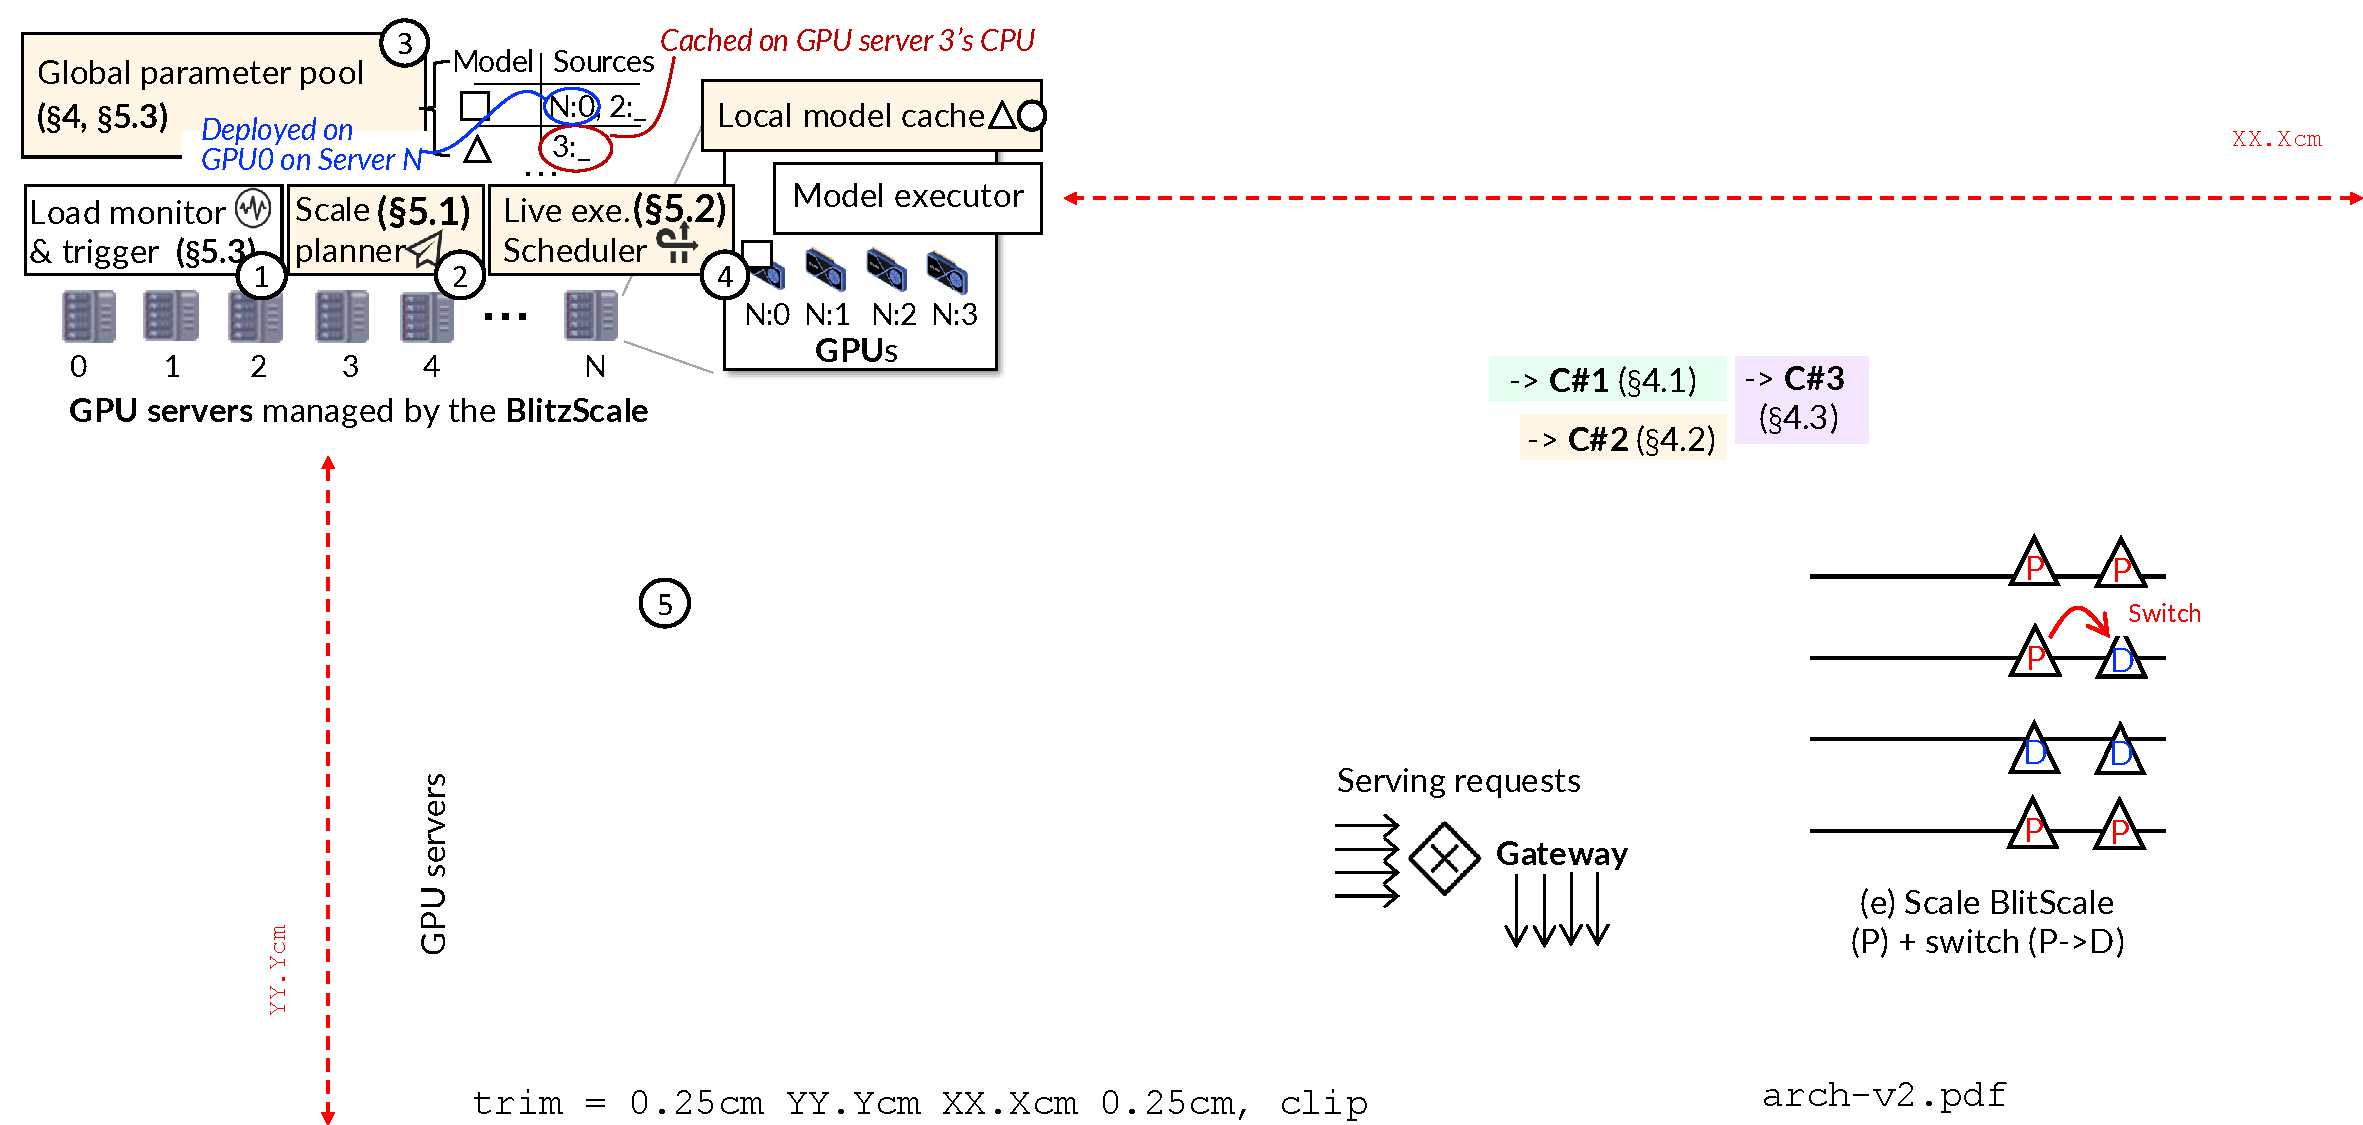
\includegraphics[width=.99\textwidth, trim=0.25cm 11.6cm 22.3cm 0.25cm, clip]{figs/arch-v2.pdf} \\[1pt]
        \end{minipage} \\[3pt]
        \begin{minipage}{1\linewidth}
        \caption{\small{\textit{
            System architecture of {\sys}.
            New modules introduced by {\sys} are marked with {\fboxtwo}. 
        }}}
        \label{fig:arch}
        \end{minipage} \\[-10pt]
        \end{figure} 

\noindent
{\sys} scales models through the compute network 
to accelerate scaling even under cache misses on the host.
We achieve this by first managing model parameters---scattered across GPUs behind serving instances
 (for deployed models) 
and CPUs (cached at the host)---through a global parameter manager. 
The manager maintains a mapping between models and their sources. 
With the manager, we can quickly read parameters from these sources with the fast 
RDMA or NVLink.
Besides, we also offload computation from overloaded instances to 
instances with partially loaded parameters to achieve live scaling.        

\stitle{System architecture and workflow. \,}
{\fig{fig:arch}} shows our system architecture.
Like prior work~\cite{DBLP:conf/usenix/Romero0YK21,DBLP:journals/corr/abs-2401-14351,DBLP:conf/osdi/SunHZXZL024},
we have a load monitor (\ding{192})
tracking the serving load for each model service,
and deciding whether to scale and how many new instances are required (\textsection{\ref{sec:design-others}}).
On each machine, we further adopt off-the-shelf GPU kernels FlashInfer~\cite{flashinfer}
to query the model efficiently.
The key differences are twofold.
First, our scale planner (\ding{193}) will
derive a scaling plan that guides how to load parameters onto the scaled instances (\textsection{\ref{sec:design-plan}})
with compute network efficiently.
The planner consults the global parameter manager (\ding{194}) to identify the sources of model parameters.
In our example, the new instance can load the parameters of model {$\square$}
from the GPU0 on host N ($N,0$), or from host 2's CPU memory ($2,\_$).
Second,
during scaling,
our live execution (exe.) scheduler (\ding{195}) will redirect requests between instances to
fully utilize the scaled instances even before the parameters are fully loaded (\textsection{\ref{sec:design-pp}}).

\begin{figure}[!t]
    %    \vspace{2mm}
        \begin{minipage}{1\linewidth}
        \hspace{-1mm}
        \centering    
        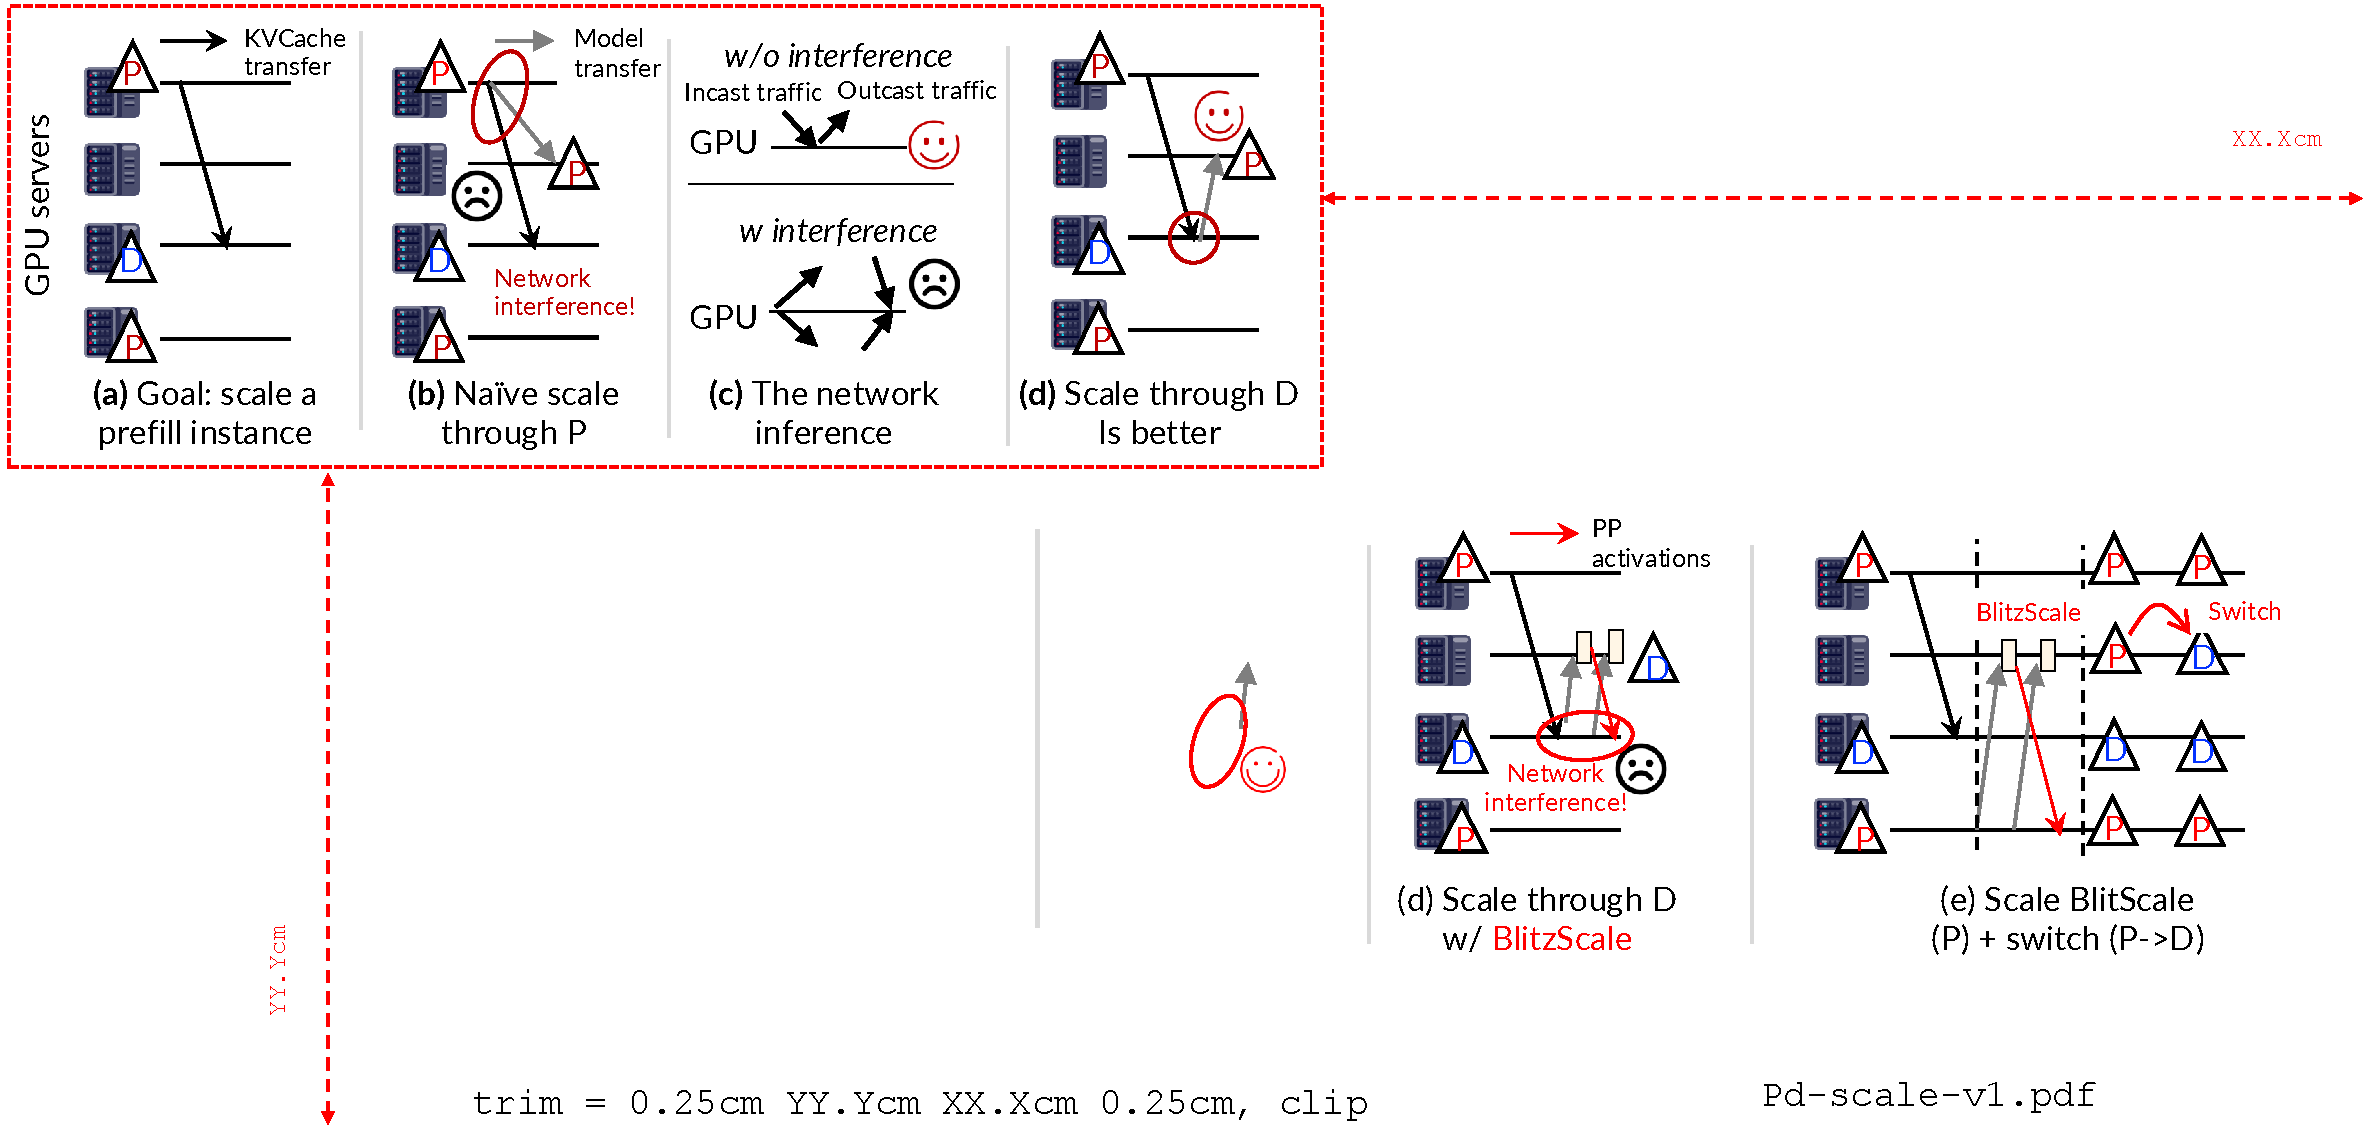
\includegraphics[width=.99\columnwidth, trim=0.25cm 11.3cm 17.7cm 0.25cm, clip]{figs/pd-scale-v1.pdf} \\[1pt]
        \end{minipage} \\[5pt]
        \begin{minipage}{1\linewidth}
        \caption{\small{\textit{
            (a) An illustration of scaling a prefill instance for LLM PD disaggregated serving. 
            (b) Naively scaling from a prefill instance imposes network interference.
            (c) Interference can be avoided by leveraging the bi-directional feature of modern DCN networking. 
            (d) An improved scale plan with the bi-directional in mind. 
        }}}
        \label{fig:pd-scale}
        \end{minipage} \\[-10pt]
        \end{figure}    
        
\begin{figure}[!t]
    \centering
    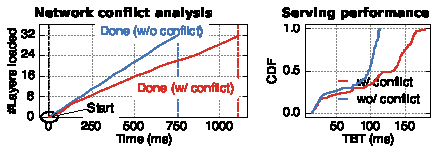
\includegraphics[left, scale=1.1]{./data/motiv-netconflict.pdf} \\[0pt]
    \begin{minipage}{1\linewidth}
            \caption{\small{\textit{
            A characterization of network interference on (a) scaling speed and (b) serving performance. 
        }}}
    \label{fig:motiv-network-conflict}
\end{minipage} \\[-5pt]
\end{figure}           


\stitle{Challenges and approaches. \,}
Despite leveraging fast networking, making autoscaling
fast and live needs to address the following challenges.

\emph{\uline{C\#1. Online interference-free scale plan generation.} \,}
Generating the scale plan is similar to generating a \emph{multicast} plan~\cite{DBLP:journals/jpdc/BhatRP03,DBLP:conf/asplos/CowanMMSX23,DBLP:conf/sc/GhazimirsaeedZR20,DBLP:conf/icpp/BanikazemiMP98,DBLP:conf/dsn/BehrensJBT18},
i.e., how to quickly distribute data (parameters) from some sources to targets.
There are two additional requirements for autoscaling.
First, the plan must be generated online on dynamically changing sources and targets,
but optimal plan generation is NP-hard~\cite{DBLP:journals/jpdc/BhatRP03} on a heterogeneous network.
Second, the plan needs to eliminate interference between loading and the serving workload.
{\fig{fig:pd-scale}} shows an example when a model is served via PD disaggregation.
In PD disaggregation serving workload KVCache is migrated from prefill to decode instances (a), 
and this migration overhead can be hidden~\cite{DBLP:conf/isca/PatelCZSGMB24}.
However, suppose we want to scale a prefill instance:
if we naively select a prefill instance as the source (b),
the scaling will compete the network bandwidth with the serving workload,
leading to 1.5\,$\times$ longer scale time as well as 50\% tail TBT increase due to the 
amplified KVCache migration overhead
({\fig{fig:motiv-network-conflict}} (b)).

To this end,
we design a serving-guided greedy plan generation method
based on three observations (\textsection{\ref{sec:design-plan}}).
First,
the network heterogeneity mainly comes from NVLink,
whose speed is extremely fast,
i.e., it can broadcast a Llama3\,8B to 8 GPUs within 120\,ms.
Thus, we can abstract instances linked with NVLink as a logical instance group
to eliminate NVLink from the network topology.
Second, loading parameters from the network is bandwidth-intensive,
so we can greedily construct serial forwarding chains~\cite{DBLP:conf/icpp/VerstoepLB96}
for multicast, which is optimal in the common case.
Finally, the network (RDMA) between GPU servers is bi-directional~\cite{288657,rdma-bidirectional},
meaning that the network flows of incast and outcast don't interfere (c).
Thus,
we can leverage this feature to avoid interference
by removing flows in the same direction on the same network link during plan generation.
For example, we can load the parameters from the decode instance to the prefill instance (see {\fig{fig:pd-scale}} (d)).

\iffalse
To address this challenge, our planner (\textsection{\ref{sec:design-plan}}) will consider 
interference when generating the scale plan, which is possible by leveraging the static dataflow 
nature of serving workloads that require extensive network usage.
While generating such a plan is not too hard, 
the design space becomes more complex when we consider live autoscale, 
which we will also address with common model serving properties. 
\fi

\begin{figure*}[!t]
    %    \vspace{2mm}
        \begin{minipage}{1\linewidth}
        \hspace{-1mm}
        \centering    
        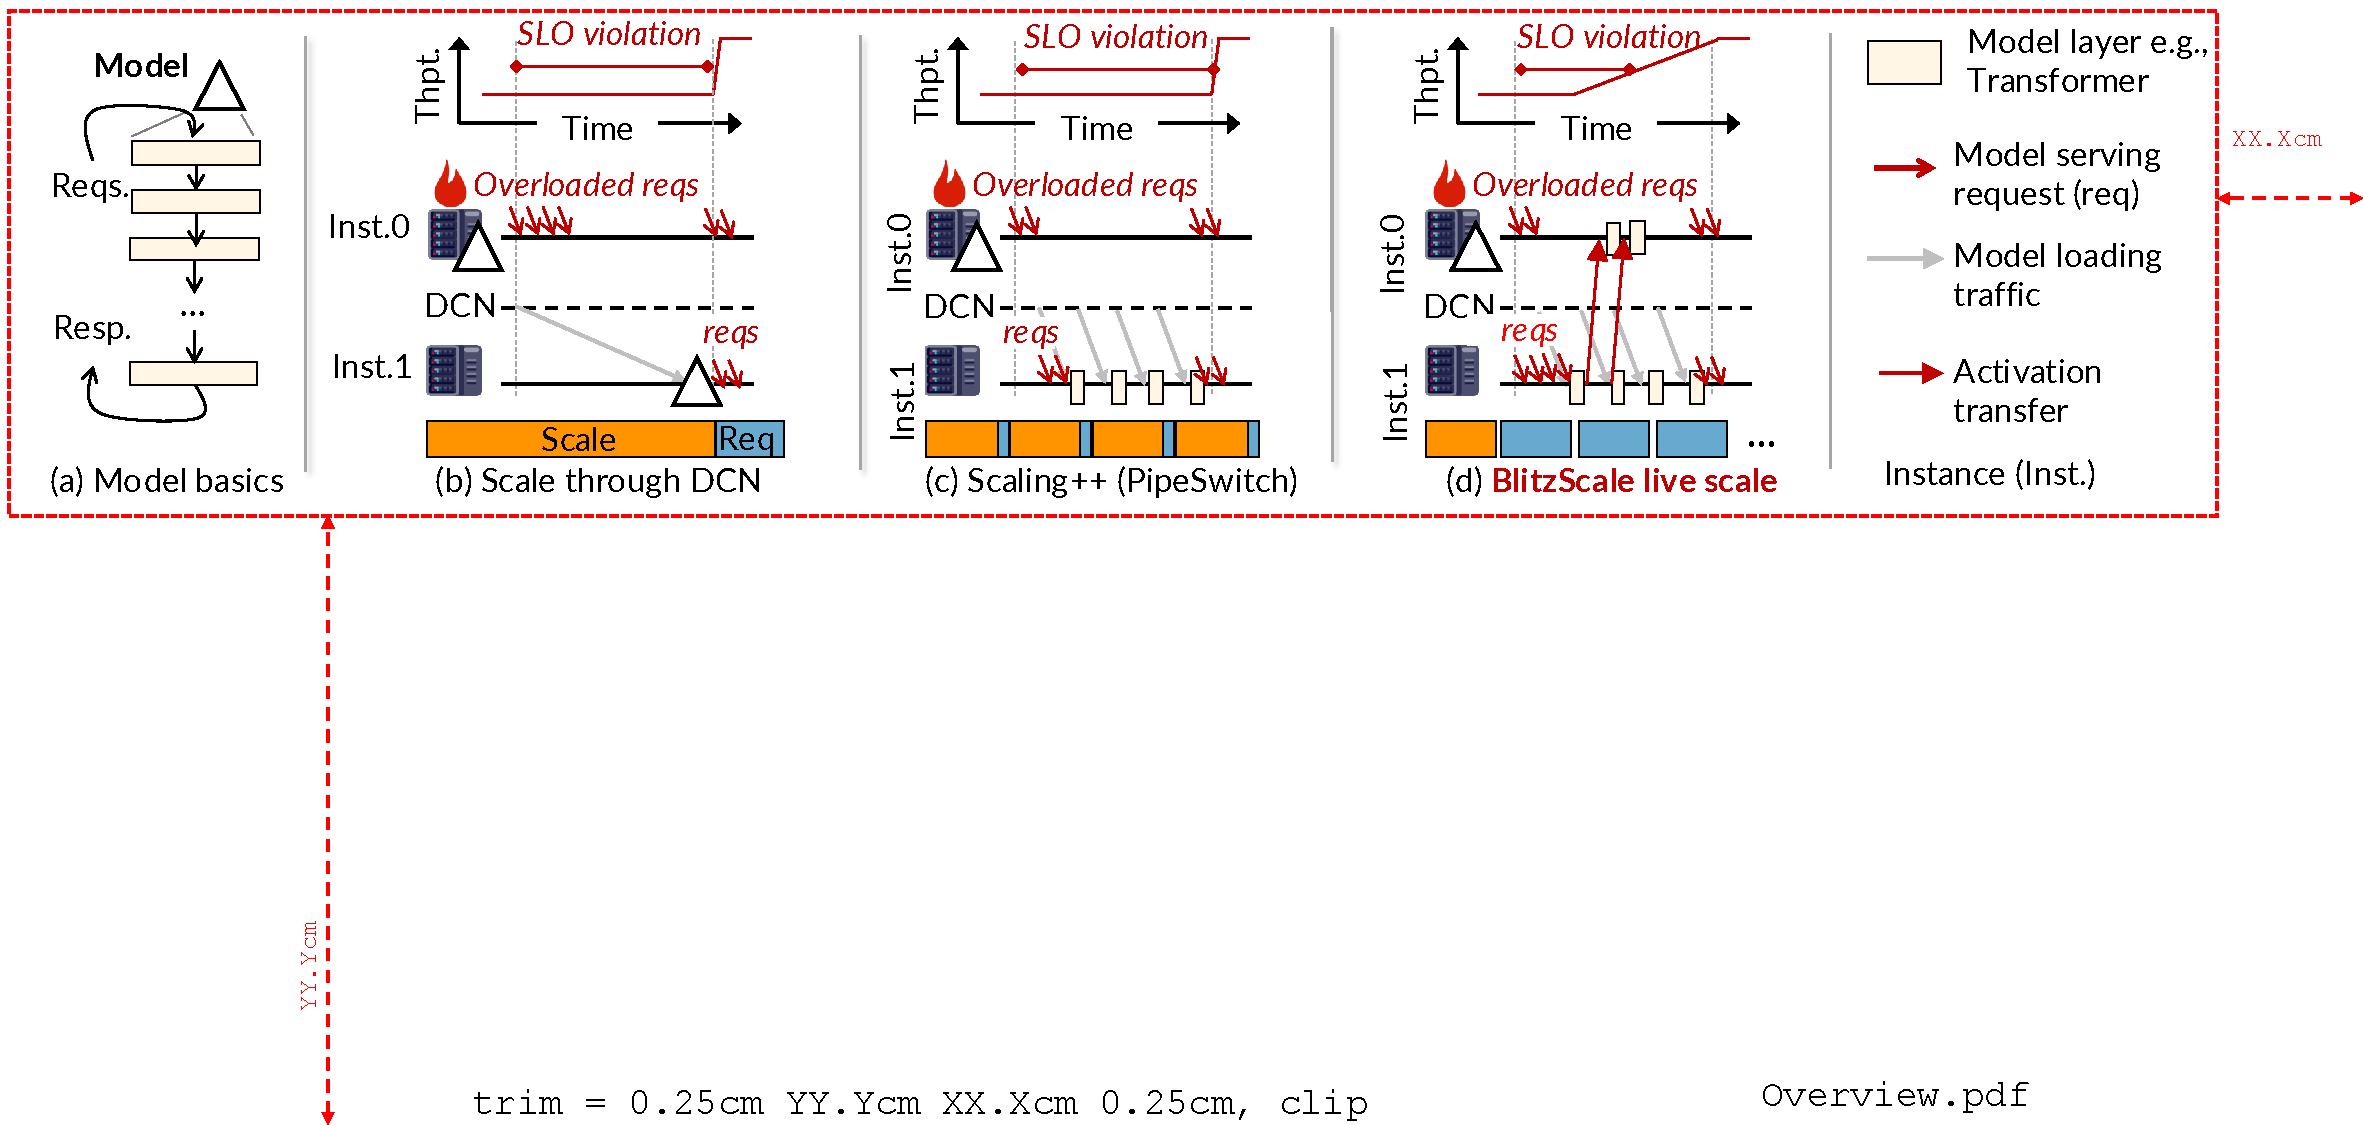
\includegraphics[width=.95\columnwidth, trim=0.25cm 10.38cm 2.5cm 0.25cm, clip]{figs/overview.pdf} 
        \end{minipage} \\[8pt]
        \begin{minipage}{1\linewidth}
        \caption{\small{\textit{
            (a) An overview of how model executes requests.
            (b) An illustration of naive model scale through DCN.
            (c) An illustration of an optimized scaling method with overlapped execution~\cite{pipeswitch},
            but it still cannot be live.
            (d) How {\sys} scales models lively.
        }}}
        \label{fig:overview}
        \end{minipage} \\[-10pt]
        \end{figure*} 

\vspace{1.ex}
\emph{\uline{C\#2. Realizing live autoscale.} \,}
Live autoscaling---allowing the scaled instance 
to increase system throughput before all parameters are fully loaded---is 
necessary because
SLO violations can still happen ({\fig{fig:motiv-scale-speed}} (c)) even with fast networking. 
It is challenging to achieve this in existing systems. 
For example, 
PipeSwitch~\cite{pipeswitch} and DeepPlan~\cite{deepplan} leverage the layer-by-layer 
execution nature of models to perform inference: 
As shown in {\fig{fig:overview}} (c), 
once the first layer is loaded on inst.1, 
they redirect the overloaded requests to it for execution. 
Meanwhile, inst.1 will load subsequent layers concurrently. 
However, such overlapping is not live 
because, until all the layers are loaded, inst.1 still cannot finish requests
to increase the system throughput.

To this end,
we propose a novel cooperative execution scheme for live autoscaling.
The key observation is that though the scaled instance alone
cannot finish the requests until all layers are loaded,
it can alleviate the load of the overloaded instance with its loaded layers,
thus improving the serving throughput.
{\fig{fig:overview}} (d) illustrates this.
When inst.0 becomes overloaded and inst.1 is under scaling,
after inst.1 has loaded the first layer,
we redirect all requests from inst.0 to inst.1 for execution.
Once inst.1 completes the first layer's execution,
it forwards the activation back to inst.0 to process the remaining layers,
and the system throughput increases with reduced queued latencies,
as queued requests are processed faster. 
To see why the throughput increases, 
consider serving a 7-layer model.
inst.0 alone will have a throughput of 1/7.
With our live scaling,
after loading one layer on inst.1,
inst.0 only needs to execute 6 layers,
so its throughput increases to 1/6.
The throughput continues to improve as more layers are loaded,
reaching the peak (doubled) after half of the layers have been loaded---half of the scaling time.
\textsection{\ref{sec:design-pp}} describes our ZigZag scheduling for coordinating overloaded
and new instances during live autoscaling to achieve optimal performance for live autoscaling.